\documentclass[a11paper]{article}
% xelatex

\usepackage{subcaption}
\usepackage{tabularx}
\usepackage{titlepage}
\usepackage{document}
\usepackage{booktabs}
\usepackage{multicol}
\usepackage{multirow}
\usepackage{float}
\usepackage{varwidth}
\usepackage{graphicx}
\usepackage{siunitx}
\usepackage{pifont}
\usepackage{subcaption}
% \usepackage[toc,page]{appendix}
\usepackage[usenames,dvipsnames]{xcolor}

\title{Rapport d'APP}

\class{Logique Combinatoire}
\classnb{GEN420 \& GEN430}

\teacher{Berthié Gouin-Ferland \& Nikola Zelovic}

\author{
  \addtolength{\tabcolsep}{-0.4em}
  \begin{tabular}{rcl} % Ajouter des auteurs au besoin
      Benjamin Chausse & -- & CHAB1704 \\
      Shawn Couture    & -- & COUS1912 \\
  \end{tabular}
}

\newcommand{\todo}[1]{\begin{color}{Red}\textbf{TODO:} #1\end{color}}
\newcommand{\note}[1]{\begin{color}{Orange}\textbf{NOTE:} #1\end{color}}
\newcommand{\fixme}[1]{\begin{color}{Fuchsia}\textbf{FIXME:} #1\end{color}}
\newcommand{\question}[1]{\begin{color}{ForestGreen}\textbf{QUESTION:} #1\end{color}}

% Checkboxes
\setlength{\fboxsep}{1pt}
\newcommand{\cbox}{\fbox{\phantom{\ding{51}}}}
\newcommand{\cboxtick}{\fbox{\ding{51}}}%

\newcommand{\quicktable}[4]{
  \begin{table}[H]
    \footnotesize
    \centering
    \caption{#1}
    \label{tab:#2}
    \begin{tabular}{#3}
      #4
    \end{tabular}
  \end{table}
}

\newcommand{\quickfigure}[4]{
  \begin{figure}[H]
    \centering
		\includegraphics[width=#3\textwidth]{#4}
    \caption{#1}
    \label{fig:#2}
  \end{figure}
}

\begin{document}
\maketitle
\newpage
\tableofcontents
\newpage

\note{Un total de 4 pages est permis, excluant la page titre, la table des matières, l'introduction,
la conclusion et les références.}

\section{Introduction}

Dans le cadre de l'APP2 de la session S4, il est demandé de compléter le
développement d'une pédale d'effets de guitare numérique à l'aide d'un FPGA
sur la carte Zybo. Plus précisément, ce rapport documente la conception,
l'implémentation et la vérification de deux modules essentiels au système:
le décodeur I2S (M1), responsable de la désérialisation du signal audio reçu,
et le module de calcul de la puissance du signal (M6). Ces travaux ont été
réalisés en respectant les contraintes de synchronisation, de modularité et
de formalisme en VHDL, selon les normes enseignées. Le rapport présente les
diagrammes d'états, les schémas-blocs, les plans de vérification ainsi que
les résultats de simulation attestant de la conformité fonctionnelle des
modules développés.

\section{Module M1}
\quicktable{Plan de vérification du module M1 -- décodeur I2S}{mef-m1}{p{4cm}p{5cm}p{6cm}l}{

  \toprule
  \textbf{Objectif Ciblé} & & \textbf{Valider la MEF décodeur I2S} & \\
  Condition à proscrire & Aucune & & \\
  \midrule
  \textbf{Test} & \textbf{Action} & \textbf{Résultat attendus} & \cboxtick \\
  \midrule

  Condition initiale
  & Aucune
  & Les registres et échantillons sont à $0$.
  & \cbox \\

  Reset initial
  & \texttt{BTN3} à $1$
  & Les registres restent à $0$ peut importe la valeur des échantillons.
  & \cbox \\

  Envoie répétitif du même code au même channel. (droite)
  & Envoie de 4x \texttt{0xF0F0F0} au channel droit (.txt)
  & \texttt{0xF0F0F0} est lu sur le registre de droit pour la durée de 4 affichages.
  & \cbox \\

  Envoie répétitif du même code au même channel. (gauche)
  & Envoie de 4x \texttt{0xF0F0F0} au channel gauche (.txt)
  & \texttt{0xF0F0F0} est lu sur le registre de gauche pour la durée de 4 affichages.
  & \cbox \\

  Test de messages mix (droite)
  & Envoie de suites d'ondes à fréquences qui augmentent au channel droit (.txt)
  & Les échantillons sont présentés à la sortie du registre de droit sans changement.
  & \cbox \\

  Test de messages mix (gauche)
  & Envoie de suites d'ondes à puissances qui augmentent au channel gauche (.txt)
  & Les échantillons sont présentés à la sortie du registre de gauche sans changement.
  & \cbox \\

  Test de reset en pleine lecture
  & Envoie d'onde constantes aux deux channels, appui sur BTN3 en pleine lecture.
  & Les sorties des registres tombent à 0. La lecture recommence lorsque \texttt{LRC} change de front.
  & \cbox \\

\bottomrule
}

\quickfigure{Machine à états finis du module M1}{mef-m1}{}{assets/m1-mef-mermaid.pdf}

\begin{figure}[H]
  \centering
  \begin{subfigure}{.496\linewidth}
    \centering
    \includegraphics[width=\textwidth]{assets/chrono-m1-reset-works-awaits-LRC-change.png}
    \caption{Fonctionnement du reset et attente du changement de LRC}
    \label{fig:chrono-m1-reset-works-awaits-LRC-change}
  \end{subfigure}
  \begin{subfigure}{.496\linewidth}
    \centering
    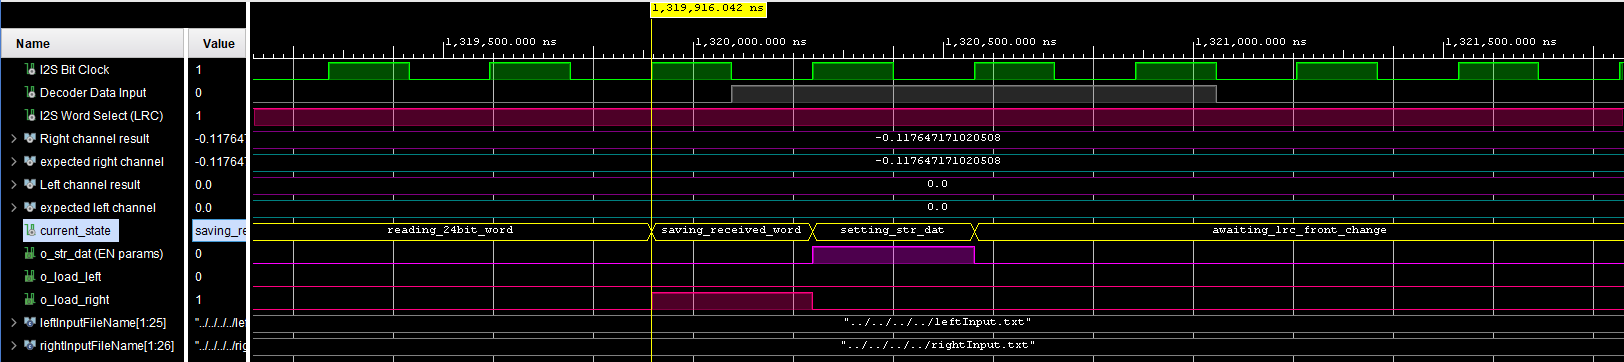
\includegraphics[width=\textwidth]{assets/chrono-m1-param-enable-reg-activation-return-await.png}
    \caption{Activation des registres et retour à l'état d'attente}
    \label{fig:chrono-m1-param-enable-reg-activation-return-await}
  \end{subfigure}
  \begin{subfigure}{.496\linewidth}
    \centering
    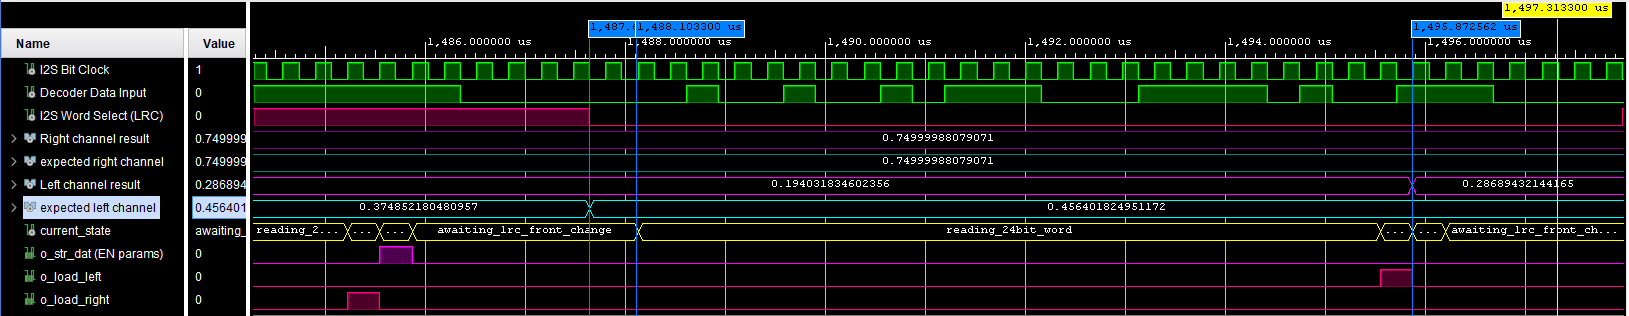
\includegraphics[width=\textwidth]{assets/chrono-m1-detect-change-LRC-save-output-to-channel.png}
    \caption{Détection du changement de LRC et enregistrement des données dans le canal approprié}
    \label{fig:chrono-m1-detect-change-LRC-save-output-to-channel}
  \end{subfigure}
  \begin{subfigure}{.496\linewidth}
    \centering
    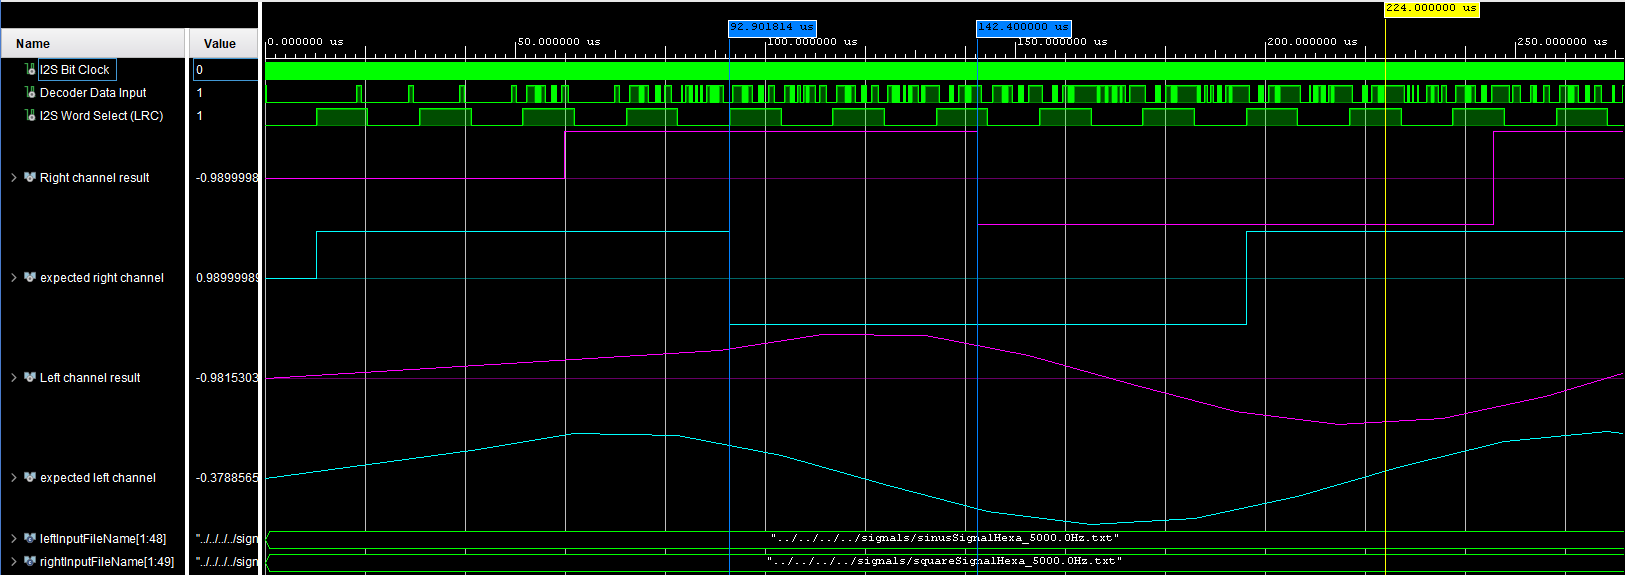
\includegraphics[width=\textwidth]{assets/chrono-m1-input-becomes-output.png}
    \caption{Conversion des données de sérial en entrée à parallèle en sortie}
    \label{fig:chrono-m1-input-becomes-output}
  \end{subfigure}
  \caption{Chronographes du module M1 sous différentes conditions}
\end{figure}





\note{votre lecteur ne connait pas votre démarche ni
pourquoi un tel résultat démontre le bon fonctionnement – vous devez l'expliquez brièvement.}

\note{Nous ne consulterons pas le dépôt de vos fichiers Xilinx (sauf
dans des cas particuliers) ce qui signifie que votre rapport doit être complet en lui-même.}

\subsection{Description du fonctionnement}

Le décodeur I2S détecte et extrait les échantillons stéréo (gauche et droite)
transmis en série par le CODEC audio via le protocole I2S. Son
fonctionnement repose sur une machine à états finis synchronisée par
l'horloge bit \verb|i_bclk|.\\

Le module débute dans l'état \verb|awaiting_lrc_front_change|, où il détecte
une transition sur le signal de sélection de mot \verb|i_lrc|. Lorsqu'une transition
est détectée, le compteur de bits et le registre à décalage sont réinitialisés,
et l'état passe à \verb|reading_24bit_word|.\\

Dans cet état, les bits sont captés en série à chaque front d'horloge et
décalés dans un registre. Une fois 23 bits reçus (le bit 0 étant le premier),
le décodeur passe à l'état \verb|saving_received_word|, où il déclenche le chargement
du mot complet dans un registre parallèle : vers \verb|o_load_left| si le mot
correspond au canal gauche (\verb|i_lrc| = 0), ou vers \verb|o_load_right| si
c'est le canal droit (\verb|i_lrc| = 1).\\

Finalement, l'état bascule à \verb|setting_str_dat| et active le signal \verb|o_str_dat| si le mot
appartient au canal droit. Ce signal sert à synchroniser les modules en aval,
comme les fonctions de calcul de puissance et de fréquence, qui ne s'appuient
que sur les échantillons du canal droit. Le système revient ensuite à l'attente
d'une nouvelle transition sur \verb|i_lrc|.\\

Les chronogrammes fournis ont été fait à l'aide du banc de test fourni. Quelques noms de certains signaux ont été changés afin d'être intuitif. 
Le chronogramme A démontre l'activation du bon registre \verb|o_load_right| si \verb|lrc| est à $1$ et le tout dans les bons états (jaune). Le chronogramme B 
démontre à l'aide de curseur les moments précis ou la lecture sur 24 bits est effectués. Autrement dit, un cycle complet de la machine à états. Ont voit le 
changement de LRC et la lecture qui commence une monté d'horloge plus loin. Le chronogramme C démontre que les signaux qui sorte du décodeur sont les mêmes
que les signaux qui entre dans le banc de test. Le décalage des ondes s'explique par le fait qu'elles doivent passé dans le codeur avant le décodeur et ces
exécutions prennent plusieurs coup d'horloge de délai. Finalement, le chronogramme A démontre le fonctionnement du reset. Tout est à zéro temps que le bouton
est appuyé et la lecture recommence uniquement lors du changement de LRC après l'arrêt du signal de reset.

\todo{Validation via une simulation avec le banc de test fourni. Vous devez démontrer le
fonctionnement de vos modules au travers de simulations et expliquez en quoi vous
répondez aux spécifications. Faites bon usage des curseurs, formattage des données et
agrandissements pour appuyer vos propos.}

\section{Module M6}

\note{votre lecteur ne connait pas votre démarche ni
pourquoi un tel résultat démontre le bon fonctionnement – vous devez l'expliquez brièvement.}

\note{Nous ne consulterons pas le dépôt de vos fichiers Xilinx (sauf
dans des cas particuliers) ce qui signifie que votre rapport doit être complet en lui-même.}

\quickfigure{Machine à états finis du module M6}{mef-m6}{}{assets/m6-mef-mermaid.pdf}

\todo{Schéma-bloc du système}

\subsection{Description du fonctionnement}

Le module M6 effectue une estimation de la puissance du signal audio en
appliquant une moyenne glissante exponentielle sur les échantillons entrants.
Le calcul est déclenché à chaque front montant de l'horloge \verb|i_bclk|, si
le signal d'activation \verb|i_en| est à 1.\\

À chaque activation, la puissance instantanée est obtenue en élevant au carré
l'échantillon courant \verb|i_ech|. Cette valeur est ensuite combinée avec la
puissance historique pondérée, laquelle est approximée par un facteur de
31/32 via un ensemble de décalages binaires successifs (équivalent à un
filtrage passe-bas exponentiel).\\

Le résultat de cette moyenne glissante est accumulé dans le registre
\verb|oldest_power|, et la sortie \verb|o_param| correspond à une portion des
bits de poids fort de cette somme, servant d'estimation compacte de la
puissance audio pour affichage ou traitement subséquent.\\

% \todo{Description sommaire du fonctionnement}
\todo{Plan de vérification}

\todo{Validation via une simulation avec le banc de test fourni. Vous devez démontrer le
fonctionnement de vos modules au travers de simulations et expliquez en quoi vous
répondez aux spécifications. Faites bon usage des curseurs, formattage des données et
agrandissements pour appuyer vos propos.}


\section{Conclusion}
\todo{write the fucking thing}

\end{document}
